\documentclass[aspectratio=169, 11pt]{beamer}

% --- Packages & Setup ---
\usepackage[utf8]{inputenc}
\usepackage[T1]{fontenc}
\usepackage{helvet}
\renewcommand{\familydefault}{\sfdefault}
\usepackage{xcolor}
\usepackage{booktabs}
\usepackage{graphicx}
\usepackage{tikz}
\usetikzlibrary{calc,positioning,fit}

\graphicspath{{../}{./}}

% --- Branding Colors ---
\definecolor{amritaMaroon}{HTML}{A4123F}

% --- Theme Setup ---
\usetheme{Madrid}
\usecolortheme[named=amritaMaroon]{structure}
\setbeamertemplate{navigation symbols}{}
\setbeamertemplate{footline}[frame number]

% Flow-diagram box style and screenshot placeholder
\tikzset{
    blk/.style={draw=amritaMaroon, very thick, rounded corners=3pt, fill=amritaMaroon!6,
                minimum height=1.3cm, text width=2.0cm, align=center, font=\small\bfseries},
    arr/.style={->, very thick, >=stealth, amritaMaroon}
}
\newcommand{\shot}[3]{\fbox{\begin{minipage}[c][#2]{#1}\centering\small\textbf{#3}\end{minipage}}}

\begin{document}

% =========================================================================
% TITLE SLIDE (Research-Based Project)
% =========================================================================
\begin{frame}
    % Corner Box Indicator
    \begin{tikzpicture}[remember picture,overlay]
        \node[fill=amritaMaroon, text=white, font=\bfseries\footnotesize, anchor=north east, rounded corners=2pt, inner sep=5pt]
        at ($(current page.north east) + (-0.2cm,-0.2cm)$)
        {Type 1: Research Project};
    \end{tikzpicture}

    \centering
    
\includegraphics[width=2.8cm]{logo.png}
    \vspace{0.1cm}

    {\large \textbf{\textcolor{amritaMaroon}{Trust-Aware Clustering and Controlled Broadcast\\for Secure IoV Communication}}} \\
    \vspace{0.05cm}
    {\footnotesize \textbf{23CSE498 -- Project Phase II (External Review)} \quad | \quad \textbf{Team Number: [Team Number]}} \\
    \vspace{0.15cm}

    % Student Table
    \begin{table}
        \centering
        \footnotesize
        \renewcommand{\arraystretch}{1.05}
        \begin{tabular}{|c|c|l|}
            \hline
            \textbf{S.No} & \textbf{Register Number} & \textbf{Student Name} \\
            \hline
            1 & [Register Number 1] & [Student Name 1] \\
            \hline
            2 & [Register Number 2] & [Student Name 2] \\
            \hline
            3 & [Register Number 3] & [Student Name 3] \\
            \hline
            4 & [Register Number 4] & [Student Name 4] \\
            \hline
        \end{tabular}
    \end{table}
    \vspace{0.1cm}

    {\footnotesize Guide: \textbf{[Guide]}, [Designation], Department of CSE} \\
    \vspace{0.1cm}
    {\scriptsize \today}
\end{frame}

% =========================================================================
% SLIDE 2: GUIDE APPROVAL EMAIL CONFIRMATION (Mandatory)
% =========================================================================
\begin{frame}{Guide Review \& Submission Approval}
    \framesubtitle{Confirmation of Project Review and Approval from Guide}
    \centering
    \fbox{\begin{minipage}[c][5.4cm]{0.94\textwidth}
        \centering
        \textbf{[Insert Screenshot of Guide Approval Email Here]} \\[0.3cm]
        {\footnotesize [Mandatory: Attach a clear, readable screenshot of the email received from your project guide approving this presentation and final review submission]}
    \end{minipage}}
\end{frame}

% =========================================================================
% SECTION 1: PROBLEM DEFINITION, RESEARCH MOTIVATION & SOLUTION DESIGN
% =========================================================================
\section{Problem \& Solution Design}

% --- SLIDE 1: PROBLEM DEFINITION & RESEARCH MOTIVATION ---
\begin{frame}{1. Problem Definition \& Research Motivation}
    \framesubtitle{Problem Statement, Identified Literature Gap \& Objectives}
    \begin{block}{Problem Statement}
        A crash alert is flooded by every vehicle. In dense traffic the copies collide, and anyone can start a fake alert.
    \end{block}

    \begin{block}{Research Gap}
        Earlier schemes either cut duplicates \emph{or} check the sender. We did not find both in one path to the RSU.
    \end{block}

    \begin{block}{Research Objectives}
        \begin{enumerate}
            \item Build the full path: vehicle $\rightarrow$ RSU $\rightarrow$ cloud.
            \item Send fewer frames than flooding and slotted 1-persistence.
            \item Stop forged alerts from low-trust vehicles.
        \end{enumerate}
    \end{block}
\end{frame}

% --- SLIDE 2: PROPOSED METHODOLOGY & OVERALL WORKFLOW (FULL-SLIDE DIAGRAM) ---
\begin{frame}{2. Proposed Methodology \& Overall Workflow}
    \framesubtitle{End-to-End System Workflow Architecture}
    \centering
    % NOTE FOR THE TEAM: replace this box with \includegraphics[height=5.2cm]{architecture.png} (eraser.io export)
    \fbox{\begin{minipage}[c][5.2cm]{0.94\textwidth}
        \centering
        \textbf{[Insert architecture diagram redrawn on eraser.io]} \\[0.3cm]
        {\footnotesize Vehicle Layer $\rightarrow$ Cluster Head path $\rightarrow$ V2I $\rightarrow$ RSU $\rightarrow$ Dissemination + Cloud}
    \end{minipage}}
    \vspace{0.2cm}

    \begin{block}{Workflow Summary}
        \small Trusted cluster heads forward first, duplicates are dropped, and the RSU records each event once.
    \end{block}
\end{frame}

% --- SLIDE 3a: METHODOLOGICAL COMPONENTS (VEHICLE SIDE) ---
\begin{frame}{3. Methodological Components -- Vehicle Side}
    \framesubtitle{From Cluster Formation to Controlled Broadcast}
    \centering
    \resizebox{0.98\textwidth}{!}{%
    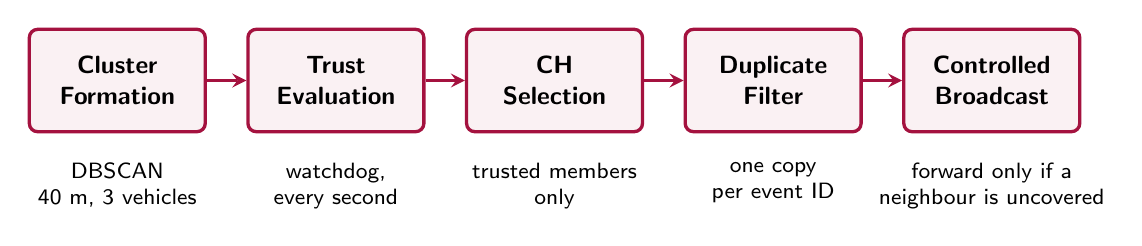
\begin{tikzpicture}
        \node[blk] (a) {Cluster\\Formation};
        \node[blk, right=0.5cm of a] (b) {Trust\\Evaluation};
        \node[blk, right=0.5cm of b] (c) {CH\\Selection};
        \node[blk, right=0.5cm of c] (d) {Duplicate\\Filter};
        \node[blk, right=0.5cm of d] (e) {Controlled\\Broadcast};
        \draw[arr] (a) -- (b);
        \draw[arr] (b) -- (c);
        \draw[arr] (c) -- (d);
        \draw[arr] (d) -- (e);
        \node[below=0.25cm of a, font=\footnotesize, align=center] {DBSCAN\\40 m, 3 vehicles};
        \node[below=0.25cm of b, font=\footnotesize, align=center] {watchdog,\\every second};
        \node[below=0.25cm of c, font=\footnotesize, align=center] {trusted members\\only};
        \node[below=0.25cm of d, font=\footnotesize, align=center] {one copy\\per event ID};
        \node[below=0.25cm of e, font=\footnotesize, align=center] {forward only if a\\neighbour is uncovered};
    \end{tikzpicture}}
    \vspace{0.5cm}

    {\large An alert spreads only after \textbf{3 trusted neighbours} sign it.}
\end{frame}

% --- SLIDE 3b: FORMULATION ---
\begin{frame}{3. Methodological Components -- Formulation}
    \framesubtitle{Governing Rules, Dataset \& Metrics}
    \begin{columns}[T]
        \column{0.56\textwidth}
        \begin{block}{Three Rules}
            \textbf{Trust}
            \[ \mathrm{trust} = \frac{s+1}{s+f+2} \qquad (\geq 0.7 \text{ is trusted}) \]
            \textbf{Wait}
            \[ T = t_{acc} + (\mathrm{tier}\cdot N_s + S(d))\,\tau + \mathrm{rand} \]
            \textbf{Forward only if}
            \[ N(v) \setminus \textstyle\bigcup_{h} \bigl(N(h)\cup\{h\}\bigr) \neq \emptyset \]
        \end{block}

        \column{0.40\textwidth}
        \begin{block}{Dataset}
            SUMO traffic, $5\times5$ grid, 2 RSUs.\\
            50--500 vehicles $\times$ 30 seeds\\
            = 180 scenarios.
        \end{block}
        \begin{block}{Metrics}
            Frames on air, receptions lost, suppression, $t_{90}$.
        \end{block}
    \end{columns}
\end{frame}

% --- SLIDE 3c: METHODOLOGICAL COMPONENTS (RSU + CLOUD SIDE) ---
\begin{frame}{3. Methodological Components -- RSU \& Cloud Side}
    \framesubtitle{From V2I to Dissemination and Cloud}
    \centering
    \resizebox{0.98\textwidth}{!}{%
    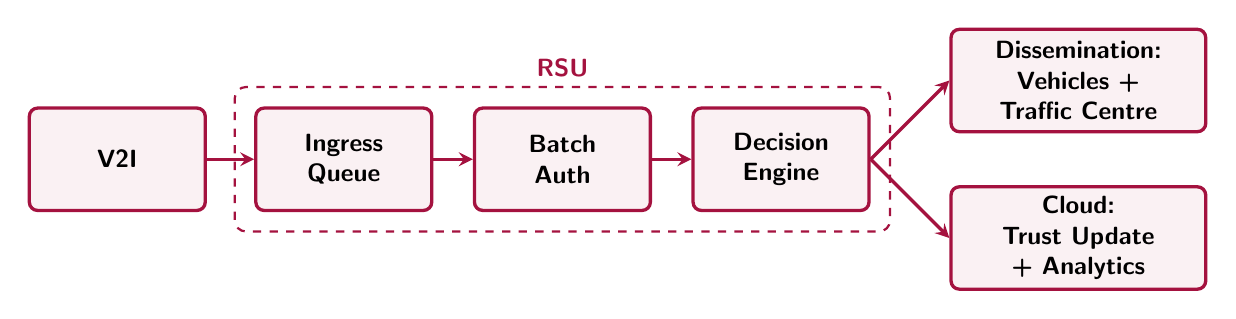
\begin{tikzpicture}
        \node[blk] (v) {V2I};
        \node[blk, right=0.6cm of v] (q) {Ingress\\Queue};
        \node[blk, right=0.5cm of q] (b) {Batch\\Auth};
        \node[blk, right=0.5cm of b] (d) {Decision\\Engine};
        \node[blk, text width=3.0cm, right=1.0cm of d, yshift=1.0cm] (o1) {Dissemination:\\Vehicles + Traffic Centre};
        \node[blk, text width=3.0cm, right=1.0cm of d, yshift=-1.0cm] (o2) {Cloud:\\Trust Update + Analytics};
        \draw[arr] (v) -- (q);
        \draw[arr] (q) -- (b);
        \draw[arr] (b) -- (d);
        \draw[arr] (d.east) -- (o1.west);
        \draw[arr] (d.east) -- (o2.west);
        \node[draw=amritaMaroon, dashed, thick, rounded corners=4pt, inner sep=7pt, fit=(q)(b)(d),
              label={[font=\small\bfseries, text=amritaMaroon]above:RSU}] {};
    \end{tikzpicture}}
    \vspace{0.5cm}

    {\large The RSU only receives. Each event is \textbf{registered once}.}
\end{frame}

% =========================================================================
% SECTION 2: IMPLEMENTATION COMPLETION
% =========================================================================
\section{Implementation Details}

% --- SLIDE 4: IMPLEMENTATION - OVERVIEW ---
\begin{frame}{4. Implementation Details -- Overview}
    \framesubtitle{Module-Wise Implementation \& Pipeline Integration Status}
    \begin{table}
        \centering
        \small
        \renewcommand{\arraystretch}{1.3}
        \begin{tabular}{p{4.6cm} p{5.4cm} c}
            \toprule
            \textbf{Module / Stage} & \textbf{Implemented in} & \textbf{Status} \\
            \midrule
            Vehicle layer, clustering, trust & \texttt{scenario.py}, \texttt{clustering.py} & Integrated \\
            Signing + controlled broadcast & \texttt{corroboration.py}, \texttt{protocols.py} & Integrated \\
            Radio channel + baselines & \texttt{channel.py}, \texttt{protocols.py} & Integrated \\
            RSU, dissemination, cloud & \texttt{rsu.py}, \texttt{infrastructure.py} & Integrated (local) \\
            Evaluation + demo & \texttt{experiment.py}, \texttt{demo.py} & Functional \\
            \bottomrule
        \end{tabular}
    \end{table}

    \begin{block}{Environment \& Repository}
        \small Python 3.11, SUMO 1.27, scikit-learn, py\_ecc (BLS), SQLite, pytest (99 tests). \\
        \texttt{github.com/AkhilRudrapaka/IoV-Emergency-Broadcast}
    \end{block}
\end{frame}

% --- SLIDE 5: CORE MODULE IMPLEMENTATION DETAILS ---
\begin{frame}{5. Core Module Implementation Details}
    \framesubtitle{Clustering and Trust in the Running System}
    \centering
    \shot{0.45\textwidth}{4.6cm}{[Insert screenshot: cluster formation in SUMO-GUI, cluster heads highlighted]}
    \hfill
    \shot{0.45\textwidth}{4.6cm}{[Insert screenshot: trust score update, per-vehicle trust before and after an event]}
    \vspace{0.3cm}

    {\normalsize Cluster heads are chosen only from vehicles with trust $\geq 0.7$.}
\end{frame}

% =========================================================================
% SECTION 3: PRELIMINARY VERIFICATION & DEMONSTRATION
% =========================================================================
\section{Verification \& Demonstration}

% --- SLIDE 6a: QUANTITATIVE RESULTS ---
\begin{frame}{6. Preliminary Verification \& Quantitative Results}
    \framesubtitle{Comparison with Existing Approaches (200 vehicles, mean of 30 runs)}
    \begin{table}
        \centering
        \small
        \renewcommand{\arraystretch}{1.3}
        \begin{tabular}{p{5.2cm} c c c c}
            \toprule
            \textbf{Method} & \textbf{Frames} & \textbf{Lost receptions} & \textbf{Suppression} & \textbf{$t_{90}$ (ms)} \\
            \midrule
            Blind flooding & 185.8 & 9632 & 0\% & 31.8 \\
            Slotted 1-persistence & 54.7 & 2070 & 73.3\% & 32.5 \\
            Slotted 1-p + random delay & 24.1 & 188 & 90.4\% & 34.0 \\
            Ours without clustering & 46.1 & 1198 & 78.2\% & 30.5 \\
            \textbf{Proposed (full)} & \textbf{26.4} & \textbf{151} & \textbf{89.1\%} & \textbf{35.3} \\
            \bottomrule
        \end{tabular}
    \end{table}

    \begin{block}{What the table shows}
        \small About 86\% fewer frames than flooding, for about 3.5 ms more delay. The best baseline is close to ours in frame count.
    \end{block}
\end{frame}

% --- SLIDE 6b: FORGED-ALERT RESULT ---
\begin{frame}{6. Preliminary Verification -- Forged Alert Test}
    \framesubtitle{Runs (out of 30) in Which Honest Vehicles Accepted a Fake Alert}
    \begin{columns}[c]
        \column{0.31\textwidth}
        \centering
        {\Huge \textbf{\textcolor{amritaMaroon}{30}}}\\[0.2cm]
        No signing

        \column{0.31\textwidth}
        \centering
        {\Huge \textbf{\textcolor{amritaMaroon}{0}}}\\[0.2cm]
        Signing + trust check,\\attacker always drops

        \column{0.31\textwidth}
        \centering
        {\Huge \textbf{\textcolor{amritaMaroon}{25}}}\\[0.2cm]
        Signing + trust check,\\attacker behaves 90\% of the time
    \end{columns}
    \vspace{0.6cm}

    \begin{block}{Honest reading}
        The trust check works only when the attacker has a poor record. A patient attacker still gets through.
    \end{block}
\end{frame}

% --- SLIDE 7: EXPERIMENTAL VISUALIZATIONS & PROTOTYPE DEMONSTRATION ---
\begin{frame}{7. Experimental Visualizations \& Prototype Demonstration}
    \framesubtitle{Comparison Graph, RSU Decision \& Cloud Analytics}
    \centering
    \shot{0.30\textwidth}{4.4cm}{[Insert screenshot: comparison graphs, frames versus vehicles]}
    \hfill
    \shot{0.30\textwidth}{4.4cm}{[Insert screenshot: RSU decision, REGISTERED / DUPLICATE / REJECTED]}
    \hfill
    \shot{0.30\textwidth}{4.4cm}{[Insert screenshot: cloud analytics, events and pending dispatch]}
    \vspace{0.25cm}

    \begin{block}{Demonstration Overview}
        \small One crash at 200 vehicles, replayed in SUMO-GUI: flooding first, then our scheme, then a forged alert.
    \end{block}
\end{frame}

% =========================================================================
% SECTION 4: TECHNICAL KNOWLEDGE & VIVA VOCE
% =========================================================================
\section{Technical Knowledge}

% --- SLIDE 8: TECHNICAL JUSTIFICATION, DESIGN TRADE-OFFS & INSIGHTS ---
\begin{frame}{8. Technical Justification, Design Trade-offs \& Insights}
    \framesubtitle{Design Choices, Trade-offs, Limitations \& Future Scope}
    \begin{columns}[T]
        \column{0.48\textwidth}
        \begin{block}{Design Choices \& Trade-offs}
            \begin{itemize}
                \item DBSCAN: no need to fix the number of clusters.
                \item BLS: many signatures, one 96-byte signature.
                \item Signing costs about 27 ms.
            \end{itemize}
        \end{block}

        \column{0.48\textwidth}
        \begin{block}{Limitations \& Future Scope}
            \begin{itemize}
                \item Simulation only, no fading.
                \item Small grid, two RSUs.
                \item Trust can be gamed by patient attackers.
                \item Next: real city map, stronger trust.
            \end{itemize}
        \end{block}
    \end{columns}
\end{frame}

% =========================================================================
% REFERENCES & THANK YOU
% =========================================================================
\section{References}
\nocite{wisitpongphan2007,kaur2024,azizi2024,naskar2025,chen2024,lopez2018}
\begin{frame}[allowframebreaks]{References}
    \footnotesize
    \bibliographystyle{ieeetr}
    \bibliography{ref}
\end{frame}

\begin{frame}
    \centering
    {\Huge \textbf{\textcolor{amritaMaroon}{Thank You}}} \\[0.4cm]
    {\large \textbf{[Questions \& Viva Voce]}}
\end{frame}

\end{document}
